%D�finir le format du document: papier, taille de police, type de document, etc.
\documentclass[a4paper, 11pt]{article}

%%%%%%%%% Packages externes utilis�s %%%%%%%%%%%%%%%%%%%
\usepackage[french]{babel}
\usepackage[latin1]{inputenc}
\usepackage[T1]{fontenc}
\usepackage{verbatim}
\usepackage{graphicx}
\usepackage{epstopdf}
\usepackage{macro}
\usepackage{algorithm}
\usepackage{algorithmic}
%\usepackage{algorithm2e}


%La mise en page du rapport, NE PAS MODIFIER.
\usepackage{geometry}
 \geometry{
 a4paper,
 left=20mm,
 right=20mm,
 top=20mm,
 bottom=20mm,
 }

%%%%%%%%% Le corps du document entre begin et end %%%%%%%%%%%%%%%%%%%
\begin{document}

%Page de garde
%%%%%%%%%%%%%%% Page de garde %%%%%%%%%%%%%%%%%%%

\begin{titlepage}{
    \begin{center}
        \vspace* {25mm}
        {\Large \textbf {Universit� de Cergy-Pontoise}} \\
        \vspace* {10mm}
        {\Large \textbf {RAPPORT}} \\
        \vspace* {10mm}
        pour le projet de d�veloppement web \\
        \textbf {Licence d'Informatique deuxi�me ann�e} \\
        \vspace* {10mm}

	sur le sujet \\
        \vspace* {10mm}
	{\Huge \textsf{Conception d'un site web agr�gateur de donn�es}} \\
        \vspace* {10mm}
 	r�dig� par \\
        \vspace* {10mm}
        {\Large \textbf {GERARD Quentin et VILAIN Matthieu}} \\
				\vspace* {10mm}
				\noreffig{img/titre.png}{12.82cm}{8.2cm} \\
        \date Mai 2017
        \vspace* {10mm}
	\end{center}
}
\end{titlepage}


%G�n�ration automatique de la table des mati�res, de la liste des figures et de la liste des tableaux
\tableofcontents
\listoffigures
\listoftables

%Une section "remerciements" pourrait �tre int�ressante. C'est une section non num�rot� (avec un * )
\section*{Remerciements}
Les auteurs du projet voudraient remercier M.Lemaire et JL.Bourdon.

\newpage
\section{Introduction}
\label{sec:introduction}

%Il n'y a pas d'espace au d�but du paragraphe.
\paragraph{}Dans le cadre du module de de Developpement Web du second Semestre de L2, les �tudiants doivent r�alis� en bin�me un projet en r�utilisant les �l�ments appris en cours. 
Le projet consiste en la r�alisation d'un site web permettant la mise en valeur et la recherche dans les donn�es publiques de l'ONISEP, concernant les �tablissements d'enseignements sup�rieur en France.
Notre bin�me est compos� de Matthieu VILAIN, �tudiant en L2 CMI SIC, et de Quentin GERARD �tudiant en L2 CMI SIC.

\subsection{Cahier des charges}

\paragraph{Objectif}{}
Cr�er un site web agr�gateur de donn�es sur les �tablissement sup�rieur fran�ais avec recherche et tri multi-crit�res.

\paragraph{Contraintes}{}
\begin{itemize}
 \item Utiliser les donn�es des fichiers .csv ou .xml
 \item Mettre en place une recherche de donn�es
 \item Mettre en place un syst�me de tri des donn�es
 \item Afficher des statistiques sur les donn�es sous forme de graphique
 \item Mettre en place un syst�me d'historique en utilisant les cookies
\end{itemize}
Le site devra �tre disponible sur le serveur web de l'universit�. 
Il devra �galement �tre valide HTML5 et CSS3.

\paragraph{Acc�s au site}
Vous pouvez acceder au site en suivant l'un de ces deux liens :
\begin{itemize}
 \item http://projetwebmg.16mb.com
 \item https://10.40.128.22/~qgerard/projetWeb
\end{itemize}

\section{Architecture du site web}
\label{sec:architecture}

\paragraph{}Dans cette section, nous pr�sentons l'architecture du site web r�alis�.
\subsection{Architecture physique}
\label{sec:archiphys}

\paragraph{} L'architecture physique du site web est divis� en 4 parties:
\begin{itemize}
\item Les pages web: � la racine du site web
\item Les fonctions php: dans les librairies dans le dossier "lib" ainsi que dans le dossier "include"
\item Les differentes ressources: dans les dossier "res" et "img"
\item Le style du site: dans les dossier "css" et "police"
\end{itemize}

\begin{figure}[H]
	\centering
		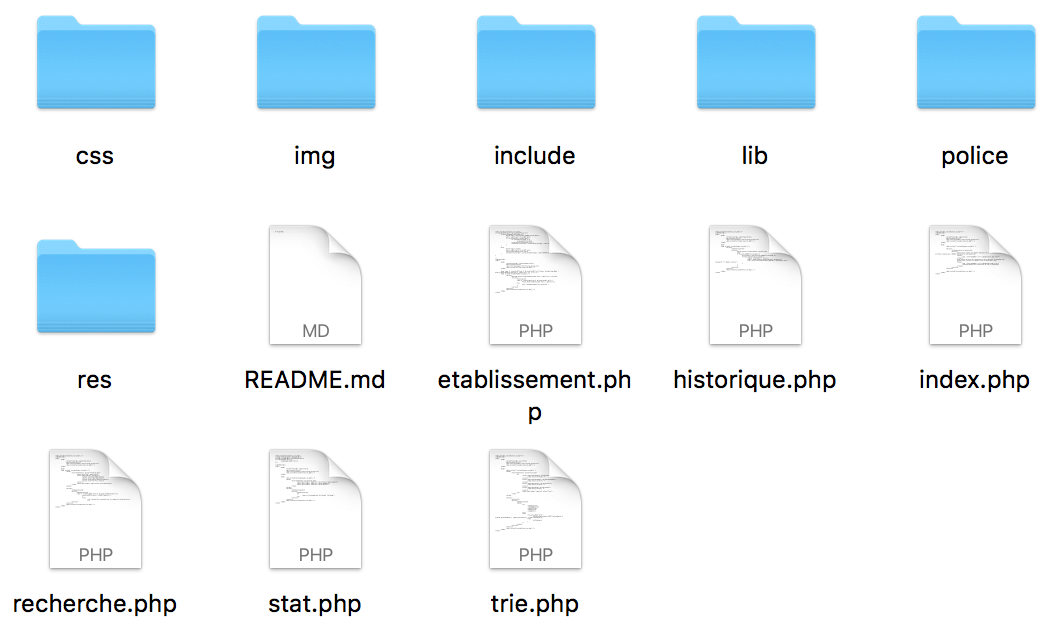
\includegraphics[width=0.75\textwidth]{img/archi_phys.png}
		\caption{Architecture Physique du site web}
	\label{fig:archiphys}
\end{figure}

\subsection{Architecture Logique}
\label{sec:archilog}

\paragraph{}Le site web est construit de telle mani�re � ce que chaque page soit accessible � partir de n'importe quelle autre page. Aisni chaque page est directement accessible via la barre de navigation pr�sente en haut de chaques pages, seule la page "�tablissement" est accessible via un lien pouvant �tre obtenu par une recherche d'�tablissement, un tri ou sur l'historique.

\begin{figure}[H]
	\centering
		
\includegraphics[width=0.75\textwidth]{img/header.png}
		\caption{Barre de navigation}
	\label{fig:navbar}
\end{figure}

\begin{figure}[H]
	\centering
		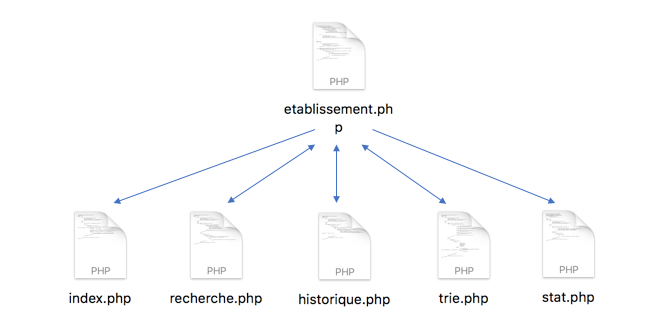
\includegraphics[width=0.75\textwidth]{img/archi_log.png}
		\caption{Architecture Logique}
	\label{fig:archilog}
\end{figure}
\newpage
\section{Choix Techniques}
\label{sec:choix}

\subsection{Type de fichier}
\label{sec:file}

\paragraph{}Pour ce projet nous avions le choix entre 2 types de fichiers pour le stockage de la base de donn�es:
\begin{itemize}
\item Extensible Markup Language (XML)
\item Comma-separated values (CSV)
\end{itemize}

\paragraph{}Nous avons choisi d'utiliser un fichier CSV pour stocker notre jeu de donn�es, et ainsi r�utiliser les connaissances accquises en cours.

\subsection{Charte graphique}
\paragraph{}Notre site web se veut sobre, �l�gant et intuitif, c'est pour quoi nous avons utilis� une palette de couleur assez sobre et pas trop vive. Le bleu est tr�s pr�sent sur notre site web, en effet c'est une couleur sobre, minist�riel, qui instaure un s�rieux, ce qui cr�� une coh�rence avec l'objet du site web.
\begin{figure}[H]
	\centering
		
\includegraphics[width=0.75\textwidth]{img/palette.png}
		\caption{Palette de couleur du site web}
	\label{fig:palette}
\end{figure}
\paragraph{}Les polices d'�critures utilis� reste dans cette m�me id�e de rester sobre, c'est pourquoi nous avons choisi d'utiliser les polices:
\begin{itemize}
\item Sansation
\item Avenir
\item Et Trebuchet MS
\end{itemize}
\newpage
\section{D�roulement du projet}
\label{sec:deroulement}

\noindent Dans cette section, nous d�crivons comment la r�alisation du projet s'est d�roul�e au sein de l'�quipe de projet. 

\subsection{Synchronisation du travail}
\label{sec:synchro}

\paragraph{}Afin de synchroniser notre travail, nous avons utilis� Git accompagn� de la plateforme GitHub.

\subsection{R�partition du travail}
\label{sec:repartition}

\paragraph{}Le tableau qui suit est � titre indicatif, il ne refl�te pas de mani�re absolue la r�partition du travail, en effet malgr� que les taches aient �t� r�parties, nous nous sommes tout de m�me entraid�.

\begin{table}[H]
\centering
\begin{tabular} {|p{7cm}|p{7cm}|}
\hline{\centering}
\bf Matthieu & \bf Quentin \\
\hline
Tri & Recherche \\
\hline
Graphiques (Statistiques) & Historique \\
\hline
HTML & CSS\\
\hline
\end{tabular}
\caption{R�partition des t�ches}
\label{tab:repartition}
\end{table}


\end{document}
